\documentclass{beamer}

\usetheme{Boadilla}

\newcommand{\bi}{\begin{itemize}}
\newcommand{\ei}{\end{itemize}}
\newcommand{\be}{\begin{enumerate}}
\newcommand{\ee}{\end{enumerate}}
\newcommand{\bc}{\begin{center}}
\newcommand{\ec}{\end{center}}
\newcommand{\I}{\item}
\newcommand{\f}{\frame}
\newcommand{\ft}{\frametitle}

\title{Offline Software for the GlueX Experiment}
\subtitle{Fall Meeting of the APS DNP, Newport News, Virginia}
\author[M.\ Ito]{Mark M.\ Ito}
\date{October 24, 2013}
\institute[JLab]{Jefferson Lab}

\begin{document}

\f{\titlepage}

\f{
\ft{GlueX in Hall D at Jefferson Lab}
\bc
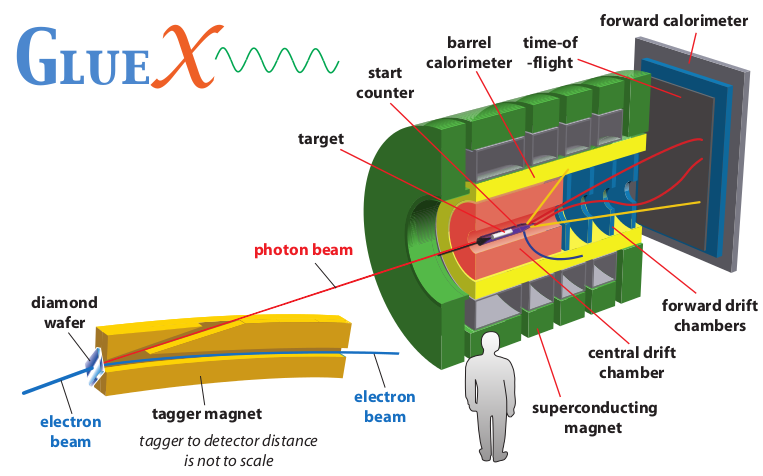
\includegraphics[height=2.9in]{Detector_withLogo.png}
\ec
}

\f{
\ft{Geometry}
\begin{columns}[c]
\begin{column}{1.7in}
  \bi\small
  \I Implemented in XML
  \I Hall D Detector Specification (HDDS)
  \I XML elements and attributes closely follow GEANT defined shapes and their parameters
  \ei
\end{column}
\begin{column}{2.8in}
  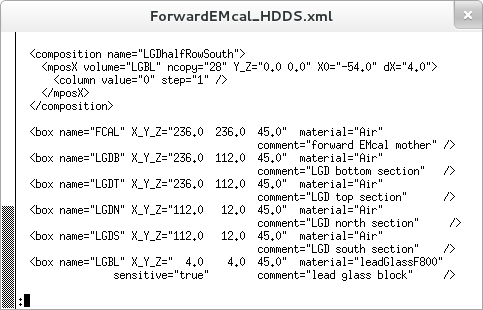
\includegraphics[width=2.8in]{hdds.png}
\end{column}
\end{columns}
  \bi
  \I Goal: keep the geometry in one place, use in
    \bi
    \I Simulation
    \I Reconstruction
    \I Event display
    \ei
  \ei
}

\f{
\ft{Simulation}
\begin{columns}[c]
\begin{column}{3.0in}
\bi
\scriptsize
\I GEANT3-based
   \bi\scriptsize
   \I Geometry defined in HDDS
   \I Out-of-time electromagnetic background included
   \I Resolution/digitization introduced in separate process (mcsmear)
   \ei
\I Geant4 Conversion
   \bi\scriptsize
   \I Well underway
   \I Geometry from same HDDS files as for GEANT3 implementation
   \I Hit generation: no new algorithms, re-use same core C code as before
   \ei
\ei
\end{column}
\begin{column}{1.5in}
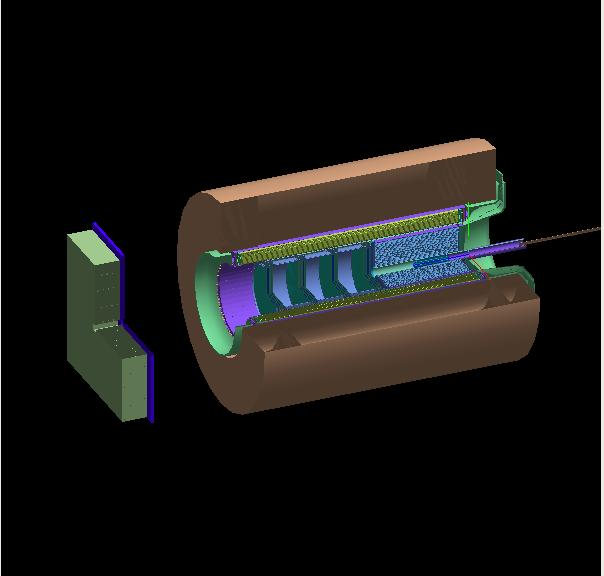
\includegraphics[width=1.5in]{cutaway.jpg}\\
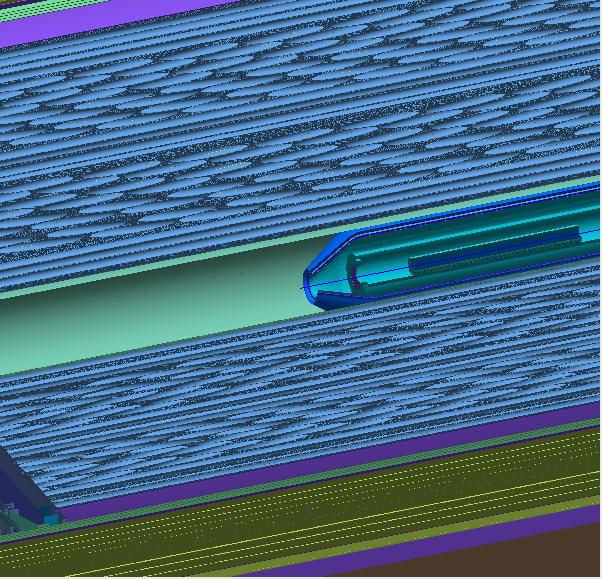
\includegraphics[width=1.5in]{cutaway_zoom.jpg}
\end{column}
\end{columns}
}

\f{
\ft{Reconstruction}
\bi
\I JANA
  \bi
  \I multi-threaded: each thread a separate event stream
  \I algorithms for different detectors implemented as "factories"
  \ei
\I ROOT used for some general utilities
\I Hooks for user code
  \bi
  \I user's class inherits from abstract base class
  \I must be registered with the framework
  \I multiple user classes possible
  \ei
\I Plug-in mechanism
  \bi
  \I e. g., define user class at run time
  \ei
\ei
}

\f{
  \ft{Amplitude Analysis}
  \bi
  \I Achieving physics goals of GlueX depends critically on amplitude analysis (partial wave analysis)
  \I AmpTools: an amplitude analysis toolkit from Indiana University
  \ei
  \begin{columns}[c]
  \begin{column}{2.0in}
    \bi
    \I event generation
      \bi
      \I hook for generating events from arbitrary amplitudes
      \I interference effect included
      \ei
    \I fitting event samples
      \bi
      \I amplitude level fits over an input event sample
      \I can be run on GPUs
      \ei
    \ei
  \end{column}
  \begin{column}{2.5in}
    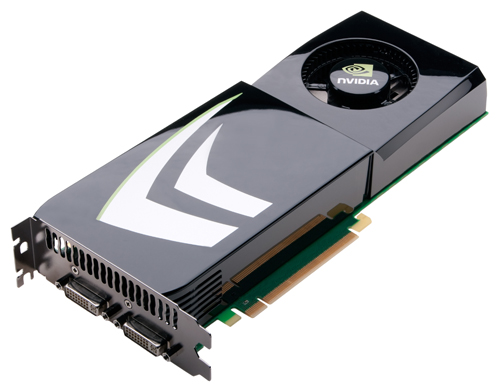
\includegraphics[width=2.5in]{GeForce_GTX_275_3qtr_large.jpg}
  \end{column}
  \end{columns}
}

\f{
\ft{Calibration Database}

\begin{columns}[c]
\begin{column}{1.7in}
\bi
\I Relational database
\I Complete version history, with version choice at API level
\I Facility for private versions, with history
\I Tagging facility
\ei
\end{column}
\begin{column}{2.8in}
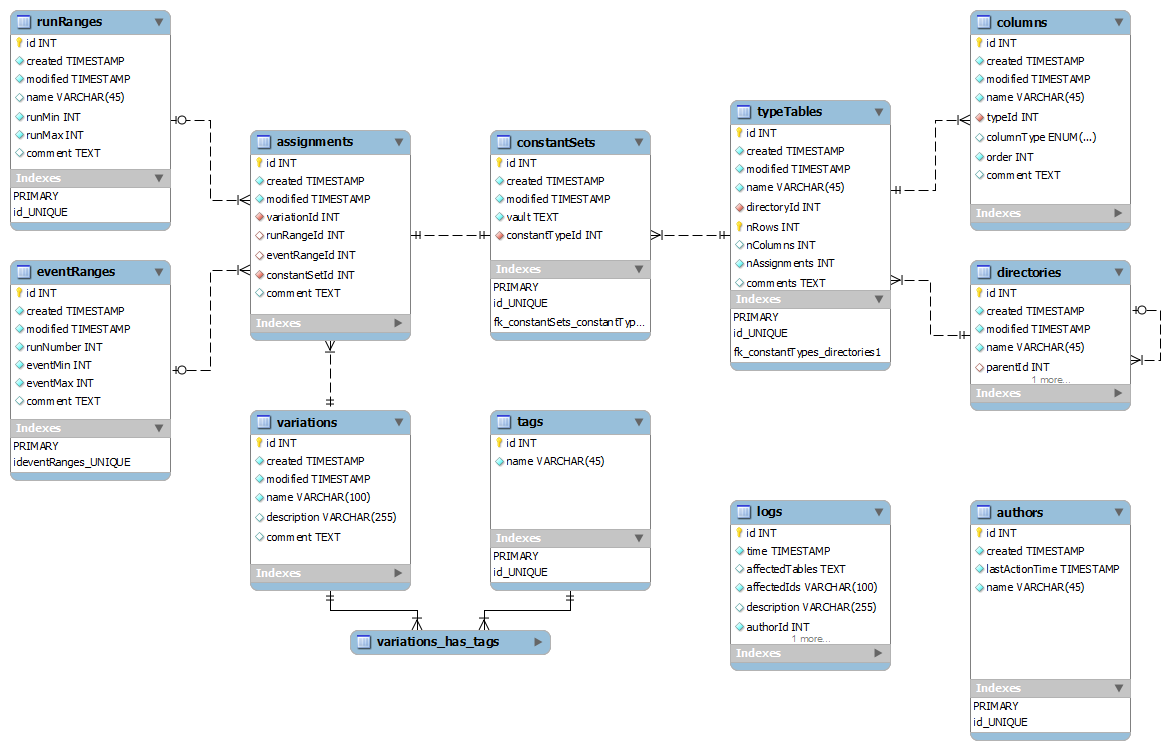
\includegraphics[width=2.5in]{schema.png}
\end{column}
\end{columns}
\medskip
\begin{columns}[c]
\begin{column}{2.25in}
Interfaces:
  \bi
  \I C++ API
  \I Web
  \I Command line
  \I Unix-like shell (CCDB shell)
  \ei
\end{column}
\begin{column}{2.25in}
Technology
  \bi
  \I Database: MySQL
  \I Reconstruction API: C++
  \I Shells and Web: Python
  \ei
\end{column}
\end{columns}




}

\f{
\ft{Data Format}

\begin{columns}[c]
\begin{column}{2.0in}
\bi\scriptsize
\I Raw data
   \bi\scriptsize
   \I EVIO: CEBAF Online Data Acquisition (CODA) format
   \ei
\I Simulated data
   \bi\scriptsize
   \I HDDM: Hall D Data Model, self-documenting on two levels
      \be\scriptsize
      \I data itself XML-like (compressed)
      \I each file contains complete mini-schema
      \ee
   \I support utilities for conversion
   \ei
\I DST data (reconstructed)
   \bi\scriptsize
   \I HDDM
   \I ROOT Trees
   \ei
\ei
\end{column}
\begin{column}{2.5in}
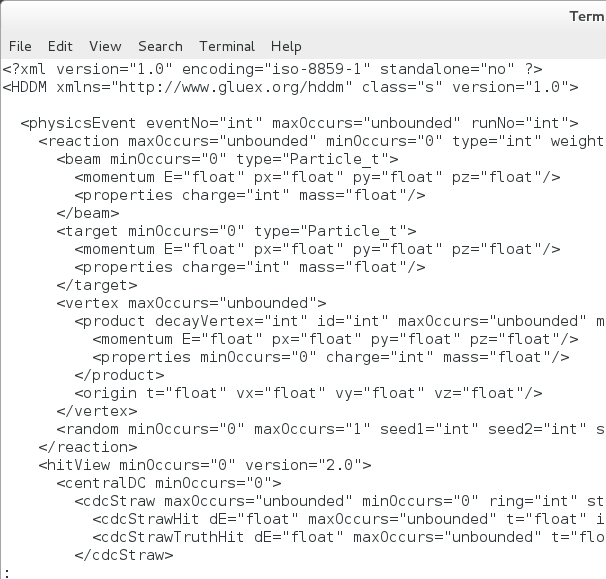
\includegraphics[width=2.5in]{hddm_template.png}
\end{column}
\end{columns}

}

\f{
\ft{Utilities}
\bi
\I XML parsing: Apache Xerces-C++
\I Source code management: subversion ($\rightarrow$git?)
\I Source code documentation: doxygen
\I Building scripts: GNU Make ($\rightarrow$SCons?)
\I Database: MySQL ($\rightarrow$MariaDB?)
\I General documentation
  \bi
  \I GlueX Notes: DocDB
  \I Webpages: mediawiki
  \ei
\ei
}

\f{\ft{CPU and Tape Requirements}
\bc
\begin{tabular}{|l|r|r|}
\hline
Process & CPU (Cores) & Tape (PB/y)\\
\hline
Raw Data & -- & 3.2 \\
Calibration & 90 & 0.06 \\
Reconstruction & 1,800 & 1.3 \\
Skims/mini-DST & 900 & 0.6 \\
Analysis & 900 & -- \\
Simulation & 5,400 & 2.5 \\
\hline
Total & 9,000 & 8 \\
\hline
\end{tabular}
\ec

\small CPU represents amount of computing power required to keep up with average rate off detector.
}

\f{
\ft{Data Challenge I}
\bi
\I Generated simulated minimum bias hadronic events
  \bi
  \I Full detector simulation
  \I Full hit-level reconstruction of simulated data
  \I Wrote out DST data
  \ei
\I November-December 2012, ran at three sites for 2 weeks
\I Event count: 5.4 billion events
  \bi
  \I Open Science Grid (OSG): 4.0 billion
  \I Jefferson Lab batch farm: 1.0 billion
  \I Carnegie Mellon Nuclear Physics Cluster: 0.4 billion
  \ei
\I About two weeks of running at 10$^7$ photons per second (coherent peak)
\I Lessons learned
  \bi
  \I jobs crash (several percent)
  \I need further development of job handling tools
  \ei
\I Data Challenge II starting November
\ei
}

\f{
  \ft{Summary}
  \bi
  \I Offline reconstruction nearly ready for data taking
  \I Large-scale data challenges very useful for insuring readiness
  \I Recent development of analysis tools:
    \bi
    \I high-level specification of reactions of interest
    \I built-in kinematic fitting
    \I event selection infrastructure (boosted decision trees)
    \ei
  \I Still more work to do:
    \bi
    \I further refinement of reconstruction
    \I further automation of production tasks
    \ei
  \ei
}

\end{document}

% end of latex file
